\chapter{Porting TinyOS for Chronos hardware}

This chapter describes the work done, to make TinyOS run on Chronos watch. Firstly, we show how we added a minimal, yet functional, platform to the OS. Then we discuss the methodology used for introducing new code. Afterwards, we go over basic MCU configuration, fundamental for other systems operation. Then we present a conceptual schema of the watch circuits that, most notably, shows connections between its elements. The remainder part of the chapter describes the hardware drivers we have created, starting with MCU internal systems and going outwards towards the peripherals.

\section{Adding a minimal functional platform}

The first milestone of our project, was to get to the point, where we could compile the \emph{Null} application and upload its image to the watch. Although this application is of little use, it does basic system initialization, therefore allowing to verify the build configuration. The additional benefit was that we could learn much about TinyOS build process.

To compile code for MSP430 architecture, we used the \emph{\bf msp430-gcc}. This was an obvious choice, because NesC compiler has built in support for it. Its installation wasn't, however, as easy as one might expect. Namely packages provided in Ubuntu were too old and did not contain headers for \emph{CC430F6137} MCU. In the end we've removed all related system packages and built the \emph{msp430-gcc} from sources, using most recent version available at the time - 4.6.2.  In addition to the compiler, tools like \emph{msp430-gdb} and \emph{mspdebug} were also installed.

The \emph{\bf mspdebug} tool is particularly important for Chronos development, as it allows to flash software on the watch through the USB debug dongle.  Additionally it also allows to debug code running on the watch, by providing a primitive gdb server, to which mentioned \emph{msp430-gdb} is able to connect\footnote{It's imperative to use the most recent version of \emph{msp430-gdb} with \emph{mspdebug}, because older versions are not compatible with it.}.

Afterwards, the {\bf NesC compiler} was installed from sources, rather than packages, followed by the TinyOS distribution. We choose a clean upstream version provided by \cite{TOSnet}. It contained some tools and scripts that also needed to be built and installed.

At this point we had a functional TinyOS installation, capable of targeting MSP430 based boards, like the \emph{telosb}. We choose to name, the new platform for our watch, \emph{chronos}. To make if fully functional, we had to create a few files under \emph{tos/platforms/chronos} path, among which only \emph{.platform} was non-trivial. This configuration file, holds various compilation parameters. In it, we had to specify the exact MCU model used in the watch, so that the generated binary images would have correct offsets for the code segment (0x8000) and the interrupt vector (0xFF80).

We also wanted the build process of an application, to be initiated with a standard TinyOS make command:
\begin{lstlisting}[numbers=none, language=bash]
  $ make chronos install
\end{lstlisting}
For this to work, we had to add a configuration file under \emph{tos/support/make} path. The \emph{chronos.target} file adds our platform to the build system, that in turn takes care of the exact NesC compiler invocations. To make the image automatically install on the device, file \emph{mspdebug.extra} was added under \emph{tos/support/make/msp} path, which invokes the commands that program Chronos.

These changes may seem obvious, but it took quite some time to work them out. Eventually we've reached the point where, the \emph{Null} application was successfully installed on the watch.

\section{Code creation methodology}

The next step, was to add the code that would make the watch operational. Generally it's considered a good programming practice to reuse existing code rather than write it from scratch. Existing code tends to be more tested and can save considerable time, especially when it contains nontrivial constructions, that would otherwise require a test and debug cycle to discover. Moreover such situations are especially frequent when dealing with hardware. Our project was quite time constrained from the beginning and various delays were to be expected further on. In these circumstances saving time wherever possible was particularly important. We benefited greatly, from the fact that TinyOS code licensing is very liberal, allowing for free use, except few very reasonable restrictions like preserving the license headers in files.

Nevertheless not all goals could be completed by adapting existing components. In such cases, where no drivers in NesC were available, we had to fall back to the hardware documentation in the form of datasheets. They describe hardware's behaviour very well, though sometimes, certain issues were only discovered and compensated for, after code was implemented and ran. As a rule, documentation very low lever, describing only control registers available on the device. All higher abstraction layers had to be devised and implemented by the developer. This is a tedious task and applying the Hardware Abstraction Architecture eases it enormously. We didn't know that from the beginning though, so some designs follow it better than others. Besides, in practice boundaries between layers aren't always clear.

Few times we encountered code that was close to what we needed, but some hardware differences made it impossible to use it directly. Modifications had to be done before it could be added to Chronos platform. In these cases we had to mix above approaches, studying the datasheets to understand inner workings of the code. However, we've found that both contributed to better understanding. Code told us much about the inner workings of the hardware and datasheets helped to understand the constructions used in the code. Most notably such approach was used to port the low level radio driver, but the principle extends to other components. As a rule, it was much easier to understand operation of a hardware device if, even a crude, driver implementation was available.

To implement the code, we first used traditional terminal based tools, like the \emph{vim} editor. Later on, when we've discovered the fine \emph{Yetti 2} plugin, we've started using \emph{Eclipse} with all its benefits. This increased our productivity considerably. Also there is no simulator of the watch available. Therefore all testing had to be done by uploading images to the hardware and observing its responses. At first we didn't even know if the programming was successful, but then when LCD display became available followed by the serial console and ultimately visual debugger, the process became quite seamless. See Appendix \ref{ch:prog_env} for details.

Finally, in what we believe is \emph{the way} to create code for mobile platforms, we tried to use \emph{TOSMOCK} for module unit-testing. This technology, however, became available too late to be widely used in our code.

\section{MCU configuration}

The MCU configuration was made much easier, thanks to the existence of a partial port of TinyOS to a similar hardware platform. The Texas Instruments \cite{EM430}, shown in Figure~\ref{fig:em430_board}, is a development board which uses the exact same \emph{CC430F6137} MCU chip as Chronos does. Work on the port was done as a part of the \cite{OSIAN} project. Though the Chronos and the EM430 differ in peripherals, much of the internal MCU configuration code was compatible and we've decided to reuse it.  Minor modification was required, to meet our coding standards and fix a few issues.
\begin{figure}[h]
  \centering
  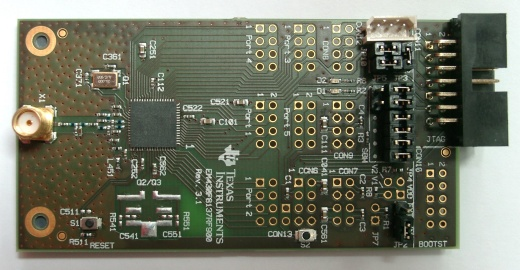
\includegraphics[width=0.7\textwidth]{img/em430_board.jpg}
  \caption{The Texas Instruments EM430F6137RF900.}
  \label{fig:em430_board}
\end{figure}

All the MCU configuration is done in the \emph{PlatformC} and the \emph{PlatformP} components, shown in Figure~\ref{fig:platformc}.
\begin{figure}[h]
  \centering
  \includegraphics[width=1.0\textwidth]{diagrams/platformc.eps}
  \caption{\emph{PlatformC} performs MCU initialization.}
  \label{fig:platformc}
\end{figure}
The first step that \emph{PlatformP} takes is disabling the watchdog. Otherwise it would shortly reset the device. Disabling it, only requires single register assignment and is done inline. In the future we may wish to use the watchdog to increase Chronos's reliability, but it wasn't a priority in this stage of the project.

One of the primary MCU responsibilities is to provide clocks and timing for other subsystems. First, let's look at the timers. In Section \ref{ch:timer_subsystem} we finished introducing TinyOS timer library, saying that the \emph{HilTimerMilliC} is provided by each platform. Continuing that discussion, Figure~\ref{fig:hil_timer_milli_c} shows a simplified structure of this component, as it is provided by the \emph{chronos} platform.
\begin{figure}[h]
  \centering
  \includegraphics[width=0.6\textwidth]{diagrams/hil_timer_milli_c.eps}
  \caption{Structure of Chronos's \emph{HilTimerMilliC}.}
  \label{fig:hil_timer_milli_c}
\end{figure}
We'll explain it's operation in bottom up order. The \emph{Msp430Timer32khzC} gives access to one of the hardware timers. \emph{Msp430AlarmC} uses it to provide an \emph{Alarm} interface with 32kHz granularity and 16 bit range. Then it is transformed by \emph{TransformAlarmC} into a wider 32 bit alarm with 1ms (actually 1024$\upmu$s) granularity. Finally, this alarm is converted into a timer and virtualized. Note that these transforming components all come from the TinyOS library.

Millisecond granularity isn't, however, sufficient for some of Chronos peripheral drivers. Delays on the order of microseconds are needed, but we didn't want to resort to active waiting. Having latency and memory footprint in mind, we decided to implement virtualized 16 bit microsecond alarms\footnote{Note, that microsecond timing is quite imprecise. Firstly it's difficult to get an event fired after less than 10$\upmu$s and the exact firing time can vary by as much as 25$\upmu$s. Still, if you need to wait 37$\upmu$s, a microsecond alarm is the best choice.} in addition to millisecond timers. They are more light-weight than timers would have been, therefore we can use them more liberally. Alarm structure is shown in Figure~\ref{fig:virutal_alarm_micro_16_c} and it's operation is similar to the timers described above.
\begin{figure}[h]
  \centering
  \includegraphics[width=0.65\textwidth]{diagrams/virutal_alarm_micro_16_c.eps}
  \caption{Structure of \emph{VirtualAlarmMicro16C} generic component.}
  \label{fig:virutal_alarm_micro_16_c}
\end{figure}

The MSP430 specific timer code comes from \emph{tos/chips/msp430/timer} library. But for CC430 MCU's, HPL layer has been overwritten with the \emph{tos/chips/msp430/msp430xv2/timer} components, which we've taken from the EM430 port.

The \emph{Msp430Timer32khzC} and  \emph{Msp430TimerMicroC} components, used above, provide access to 16 bit hardware counters Timer\_A0 and Timer\_A1, running at 32kHz and 1MHz respectively. They are implemented in this new HPL layer, but their structure is relatively simple and mundane so we will omit it. For details, see mentioned libraries.

Now we'll describe the configuration of Chronos clocks, which generate driving signals for timers and other subsystems. There are three major clocks available on the platform. The first is the {\bf REFOSC}, which uses an internal 32kHz oscillator. The second is the {\bf DCO} that uses an internal high frequency digitally-controlled oscillator, which we run at 32MHz. Third the {\bf XT1}, powered by an external 32kHz crystal oscillator. This last one supports very low power operation. MCU can be left in deep sleep state, while the external oscillator drives the clock that can then wake it. In this mode, only a tiny current is consumed. We didn't, however, utilize this option leaving it for future research.

MCU subsystems are actually fed from so called clock sources. This indirection allows to modify the clock signal before passing it on. In particular, it allows to scale down the frequency by a constant factor. There are three clock sources in CC430 MCUs. The {\bf Master Clock (MCLK)} that drives instruction execution, the {\bf Sub-System Master Clock (SMCLK)} that drives MCU peripherals and finally the {\bf Auxiliary Clock (ACLK)} that drives subsystems where slower frequencies are needed.

Clock configuration is done by the \emph{Msp430XV2ClockC} component, which is part of the \emph{tos/chips/msp430/msp430xv2/timer} library. Its structure is presented in Figure~\ref{fig:Msp430XV2ClockC}.
\begin{figure}[h]
  \centering
  \includegraphics[width=1.05\textwidth]{diagrams/Msp430XV2ClockC.eps}
  \caption{The clock configuring component.}
  \label{fig:Msp430XV2ClockC}
\end{figure}
The \emph{Msp430XV2ClockP} module configures all the clocks during its initialization. It does it through the \emph{Msp430XV2ClockControl} interface which is also made available externally, so that applications can tune the configuration if needed. Note that default MCU instruction execution speed can be modified in \emph{Msp430XV2ClockP}. This is possible, through changing the DCO frequency. \emph{Msp430XV2ClockControlP} will set MCLK to half of DCO speed, but it will always set SMCLK to 1MHz\footnote{This is one of the reasons why we drive Chronos MCU at 16MHz rather then maximum 20MHz. It is not possible to scale DCO from 40MHz to 1MHz to drive SMCLK.} and ACLK to 32kHz. Many subsystems depend on these clock sources having constant and known values. In particular, above module, also sets the Timer\_A0 to use the ACLK and Timer\_A1 to use the SMCLK. Moreover USCI uses SMCLK to drive UART, SPI and I$^2$C buses. These settings are summarised in Table \ref{fig:clock_speeds}.
The \emph{Msp430XV2ClockControlP} needs to cooperate with \emph{McuSleepC}, because of a hardware flaw present in the CC430F6137 MCUs. The workaround code needs to be notified about MCU going to sleep and waking up to calculate the sleep period length and also control the lowest sleep state that can be used.
\begin{table}
  \centering
  \begin{tabular}{ | l | l | }
    \hline
    Subsystem & Used frequency \\
    \hline
    DCO & 2MHz, 4MHz, \ldots, 32MHz \\
    REFOSC & 32kHz \\
    MCLK & DCO / 2 \\
    SMCLK & DCO scaled to 1MHz  \\
    ACLK & REFOSC \\
    Timer\_A0 & ACLK \\
    Timer\_A1 & SMCLK \\
    UART, SPI and I$^2$C & SMCLK \\
    \hline
  \end{tabular}
  \caption{Clock frequency convention used in Chronos.}
  \label{fig:clock_speeds}
\end{table}

The last action taken by the \emph{PlatformC} component is the configuration of \emph{Power Management Module}. This subsystem controls voltage fed to the MCU logic core and it needs to be increased if higher MCLK frequency is used. At lower frequencies, power can be conserved by reducing this voltage, however, setting it too low may cause unexpected behaviour. PMM can be set to one of four levels, starting with 0. Radio core can only operate at levels 2 and 3. 16MHz MCLK is also the highest frequency that can be used on PMM level 2. Therefore, we decided that it will be optimal to set it to 2.

It's worth noting, that we only noticed that PMM needs configuration after examining EM430 code. Their implementation however wasn't correct, because datasheet explicitly forbids changing the PMM level by more that one step at a time. We've corrected this in our implementation.

\section{Overview of the watch's subsystems}

In this section we present a high level schema of the Chronos systems. The Figure~\ref{fig:chronos_schema} gives a 
\begin{figure}[h]
  \centering
  \includegraphics[width=1.05\textwidth]{diagrams/chronos_schema.eps}
  \caption{Overview of Chronos subsystems and circuit board}
  \label{fig:chronos_schema}
\end{figure}
practical overview of the platform structure. The central rectangle defines the boundaries of the MCU. Beyond it, lie the external components. The connections between them, roughly present the number of wires used and more importantly, what protocol does the communication conform to. We remind that UART is the Universal Asynchronous Receiver/Transmitter and is typically used to communicate with the PC, SPI is the Serial Peripheral Interface and is used to communicate with more advanced external chips, while I$^2$C (aka. I2C) is the Inter-Integrated Circuit bus used to communicate with simpler devices, like thermometers. The IO means that the interaction is done by simply setting lines to high or low states, without using any specific communication protocol. Finally, LCD segment serialization was described in Section \ref{ch:hardware_functions}. Rectangles with bold font captions name hardware subsystem, while those with regular ones denote software components.

Rather than give brief descriptions, of each of the seven major component groups presented in the schema, and then repeat the same information in the discussion of driver code, we'll end here and refer to the schema from later sections. Finally, note, that though shown components preserve their relative structure, most have been omitted for clarity's sake.

\section{Chronos hardware drivers}

Below we describe the code that was created to make the Chronos watch operational. We go through the structure of the software of all major elements of \emph{chronos} platform, while also making notes on some of the difficulties we've encountered during our work.

\subsection{The LCD display}
Gaining access to the watch's LCD display was a vitally important step on the path of making Chronos operational.
Before that we had no way of checking if our software is actually running. There are no LEDs on its circuit board, which could normally be used to send first bits of information from the device. We did have the \emph{mspdebug} tool and the USB debug dongle, which together are capable of controlling the code execution, but reading anything from raw debug server data, proved difficult. Fortunately, a careful study of the documentation was enough to blindly configure the LCD\_B subsystem and with a bit of luck and some hours of restudying the datasheet, we managed to activate the LCD display.

Then we were gradually enhancing the driver, while progress on the rest of the project was made, until it became fully functional. In particular, it even gained the ability to display short text strings. Now we'll describe its implementation. Top level component for the LCD driver is the \emph{PlatformLCDC} shown in Figure~\ref{fig:platformc_lcd_c}.
\begin{figure}[h]
  \centering
  \includegraphics{diagrams/platform_lcd_c.eps}
  \caption{Structure of the LCD display driver.}
  \label{fig:platformc_lcd_c}
\end{figure}
Low level configuration of the refresh frequency, multiplexing, IO pin special functions, voltage control pump, internal biasing, display memory and internal voltage generation all happens in the \emph{HplCC430LCDBP} module. It provides a simple \emph{StdControl} interface to turn these settings on and off. Actual display control is implemented in \emph{LCDDriverC}, which provides the \emph{LCDDriver} interface. It is the only interface that application user cares about. This is also presented in Figure~\ref{fig:chronos_schema}.

On top of the LCD driver, the \emph{PlatformLedsC} component is built. Its structure is presented in Figure~\ref{fig:platform_leds_c}.
\begin{figure}[h]
  \centering
  \includegraphics{diagrams/platform_leds_c.eps}
  \caption{Structure of chronos abstract LEDs provider.}
  \label{fig:platform_leds_c}
\end{figure}
TinyOS libraries expect that it will provide three \emph{GeneralIO} interfaces for the LEDs and take care of initialization. \emph{LCDIconIO} generic module, adapts a specified LCD icon to the \emph{GeneralIO} interface. This an example of TinyOS Adapter design pattern, on which more can be found at \cite[ch. 8]{TOSProg}.

Finally note, that LCD driver is a poor example of HAA application, however due to its simplicity we decided that it's acceptable.

\subsection{The button support}

Buttons allow for user input during watch operation. They are, however one of these things that sound simple to implement, but are not. Problem lies in a phenomenon called bouncing, that happens when button is pressed. The metal contact isn't immediate, causing signal fluctuations preceding the state transition. Figure~\ref{fig:bouncing} illustrates this.
\begin{figure}[h]
  \centering
  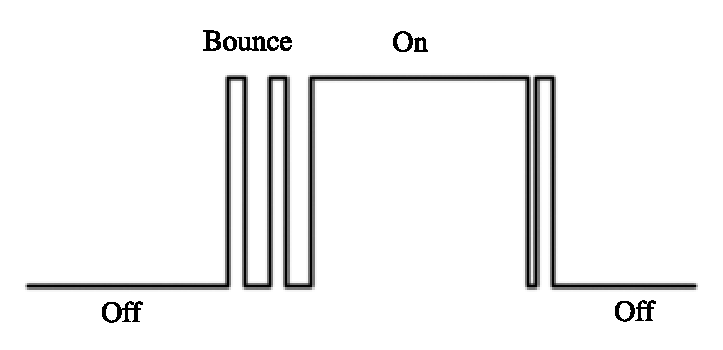
\includegraphics[width=0.6\textwidth]{img/Bounce.eps}
  \caption{Bounce effect in buttons.}
  \label{fig:bouncing}
\end{figure}
The fluctuations may cause several false press and release events. To solve this problem, so called de-bouncing is applied. This technique, measures the state of the signal several times, with each measurement separated by a short delay. Button press event is only generated if all measurements confirm that the button is pressed.

Algorithm implemented in generic component \emph{DebouncedButtonC} waits for an interrupt, notifying about button state change and then probes 3 more times during a 60ms interval. All edge cases have also been taken care of. This includes false alarms, when after the interrupt, the state doesn't seem to be changed or when the state changes just before we rearm the interrupt.

This component was made generic, because Chronos has five buttons. In Figure~\ref{fig:UpButtonC} we present the structure of one of them. All others are supported in the same way.
\begin{figure}[h]
  \centering
  \includegraphics{diagrams/UpButtonC.eps}
  \caption{The \emph{UpButtonC} abstraction.}
  \label{fig:UpButtonC}
\end{figure}
The \emph{HplMsp430GeneralIOC} and the \emph{HplMsp430InterruptC} are TinyOS library components that give access to GIO pins for MSP430 MCUs. The first provides access to pin state control, for each pin allowing to set or probe its value. The second allows to arm interrupts that fire when state of a pin changes. This is used to discover when a button is pressed.

Application using a button, can either check its state with the \emph{Get} interface or be notified about a change through the \emph{Notify} interface. Finally note, that thanks to the button independent implementations, it is possible to recognize press combinations.

\subsection{The buzzer}

Chronos has a built-in sound emitting device, called the buzzer. It can emit beeps typical to alarm clocks. The circuit that drives it is shown in Figure~\ref{fig:buzzer_circuit}.
\begin{figure}[h]
  \centering
  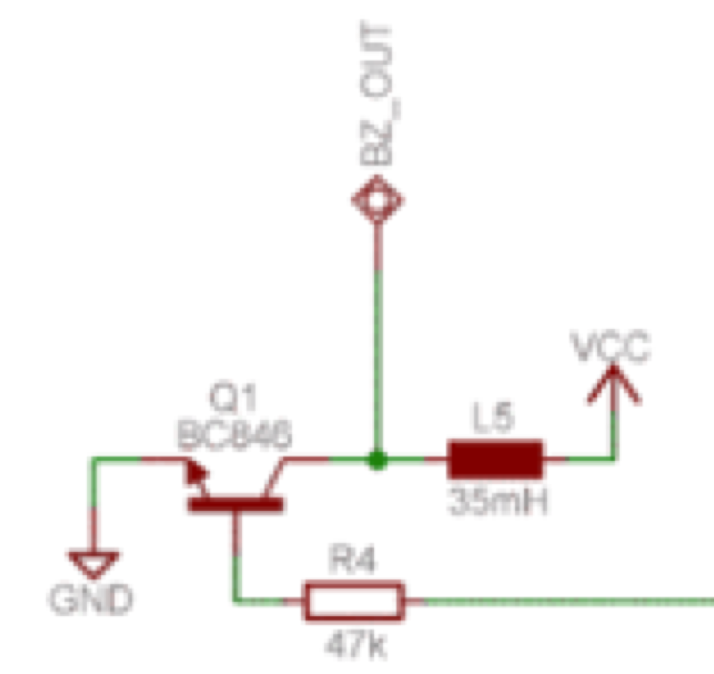
\includegraphics[width=0.30\textwidth]{img/buzzer_circuit.png}
  \caption{The buzzer circuit schema.}
  \label{fig:buzzer_circuit}
\end{figure}
The buzzer isn't connected directly to an IO pin, as Figure~\ref{fig:chronos_schema} would suggest. Instead, the IO pin triggers a transistor that really closes the buzzer circuit. 47k$\Omega$ resistor ensures that only a minimal current is drawn from the MCU. Drawing large currents from IO pins is not recommended and can be harmful. The IO pin needs to be set high, to close buzzer circuit, but this only moves its membrane one way. The L5 inductor, reverses the current running through the buzzer for a short moment after the transistor cuts the circuit, thus moving the membrane back. This way, a rectangular signal from the IO pin is transformed into sonic waves. Frequency of the waves is the same as the frequency of the signal.

We started the driver implementation by trying to actively generate this rectangular wave. Interestingly, we've found that the resulting beeps had artifacts. The tone wasn't clear. As it turned out, after disabling the interrupts the artifacts have disappeared. What we've heard, were interrupts firing and interleaving with the signal. This is the first time that we've been able to observe interrupts using human senses!

Though active signal generation, with interrupts disabled is hardly a good solution, we had neither need nor time to investigate other options. Therefore, we left the improvement of the implementation for future work. The root component of the buzzer driver is the \emph{BeeperC}, depicted in Figure~\ref{fig:buzzer_c}.
\begin{figure}[h]
  \centering
  \includegraphics{diagrams/buzzer_c.eps}
  \caption{The buzzer driver structure.}
  \label{fig:buzzer_c}
\end{figure}
It uses the \emph{BusyMicroWaitC} to generate the wave form. This is more wasteful than setting an alarm would be, but also much more precise and precision is necessary to generate a clear tone. The \emph{BeeperC} provides a simple interface, allowing to sound a single beep or a whole \emph{Power Rangers} style hail signal\footnote{It is used in the Zordon demo application.}. Though this hail is long, interrupts are only disabled while each distinct sound is emitted. This allows to process all the pending interrupts between the sounds.

Support for the Buzzer, the LCD display and the buttons allow Chronos to be a standard hand watch. Now we'll talk about more advanced features that distinguish it form such devices.


\subsection{The CC1101-based radio module}

The CC1101 is a radio transceiver chip, made by Texas Instruments. Among others, it is used in the SOWNet's \cite{G-Node} wireless sensor node, depicted in Figure~\ref{fig:gnode}. This platform is important to us, for two reasons. Firstly, a large testbed of G-Nodes has been deployed in our faculty (see \cite{MM}). Secondly, the TinyOS was ported to it by SOWNet's developers. This ensures production quality of the code and an ongoing support. Moreover, it was released on a license similar to those used in the rest of TinyOS, allowing for royalty-free use and even modification.
\begin{figure}[h]
  \centering
  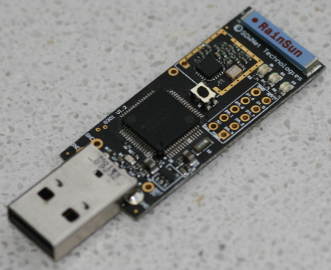
\includegraphics[width=0.5\textwidth]{img/gnode.jpg}
  \caption{The SOWNet's G-Node.}
  \label{fig:gnode}
\end{figure}
We are sure that, further research would be enhanced, if communication was possible between the watches and the G-Nodes\footnote{This way our testbed would become the largest academic deployment of wireless sensor nodes in the world, consisting of over 220 devices.}. There was no reason why it shouldn't be, because though the CC1101 radio core used to be a stand alone product, recently it was also built into the members of the CC430 family of MCUs\footnote{Credits for this are due to our project leader Konrad Iwanicki, who made the choice of hardware platforms.}. Adding this to the fact that we felt very time constrained, we've decided to adapt the G-Node's radio stack implementation, so that it could run on the Chronos. Having the same code on both types of devices, provides maximum compatibility. We also made sure that this step was legitimate by complying with the license restrictions.

We will not present the detailed structure of the radio stack, because due to its complexity, it would lie beyond the scope of this document. Besides, we were are not the authors of this code and we left most of it unchanged. We will instead focus on our porting efforts. For details on the design of the ActiveMessage communication model please refer to \cite{BHC}, \cite{TEP116} and \cite{TEP126}.

The fundamental difference between the external CC1101 core and the built-in one lies in the way they communicate with the MCU. External chip uses the SPI bus and some additional signal lines, while the internal core accepts commands through a register based interface. As we expected, almost everything else remains the same. It seems that TI has embedded the radio core into an MCU design and changed only the command interface. Our modifications follow the same pattern. We've removed all SPI related code, by deleting the whole \emph{ccpacket/spi} path and disconnecting components it contained, from the HAL layer. Then we've changed the HAL code, to send all commands through the appropriate registers. At this point, we were only missing the interrupts and the status signals that were previously generated from signal lines coming from the radio chip. Interrupts were, however, easy to replace with native ones sourced directly from the built-in core and status signals could be read from registers via query commands (or in some cases, even directly). In the end we've cleaned up the code, by removing some redundant definitions and adding comments documenting each command. Our final impression is that built-in core is easier to manage than the external one.

The bulk of these changes, was applied to \emph{HalChipconControlP} module which drives the radio core. It provides the \emph{HalChipconControl} interface, that can be used for very low level radio operation. It gives the user precise control over the transmission and reception, which might be necessary in some more sophisticated communication protocols.

During the development we've encountered some serious difficulties. The biggest delay was caused by an elusive bug, we've introduced in the code. Namely, we called an interface function, rather than a local one, that wrapped it. They had very similar names, which made the difference difficult to notice. The functions purpose was to read radio core's inner registers. However, without the use of the wrapper, few of them were read incorrectly. This caused the radio to fail in some conditions, while working normally most of the time. We spent literally weeks, trying to find the source of the instability. At this point we only had the LCD display to view state of the watch and it only supported displaying numbers. Seeing that this was getting us nowhere, we've started working on enabling the TinyOS \emph{printf} library. It helped very much, allowing us to ascertain the exact condition at which the radio failed. After some investigation, we've found that it happened during, seemingly harmless radio core register read. Finally, we've noticed the misuse. This error was very simple, but also very difficult to track down.

Another issue we've had, concerned G-Node interoperability. After porting its own radio stack to Chronos, we've expected that both will be able to communicate with each other. This wasn't the case though. We made sure that the transmission speeds matched, checked that G-Nodes are able to communicate among themselves and that Chronoses could do the same, but still they couldn't be mixed together. Finally, we've found that the problem was rooted in the \emph{support/make/chronos.target} file. Namely, it didn't contain any definition of the \emph{DEFAULT\_LOCAL\_GROUP} constant. This caused the build system to impose a default value, different from the TinyOS's default. So, both G-Node and Chronos used default value for the \emph{DEFAULT\_LOCAL\_GROUP}, but these defaults differed and nodes from different local groups ignore each others messages. We've fixed it by defining the \emph{DEFAULT\_LOCAL\_GROUP} as empty, in the mentioned file. Interestingly, an empty environment variable is treated very differently than an undefined variable. Some may view this as obvious, yet it caused us problems all the same.

Afters solving all problems, we've investigated the maximum length of the data that can be sent in one packet. In TinyOS this value is configured with the \emph{TOSH\_DATA\_LENGTH} constant. The size of the radio internal transmission/reception queue is 64 bytes. 11 are used for TinyOS packet header and 3 for the footer. This leaves safe 50 bytes for the payload. Interestingly, the radio seems to work even with this value set to 52. However we strongly recommend, never to exceed 50.

\begin{figure}[h]
  \centering
  \includegraphics[width=1.0\textwidth]{diagrams/am_sender_c.eps}
  \caption{Overview of the \emph{AMSenderC} abstraction.}
  \label{fig:am_sender_c}
\end{figure}

Finally, note that the radio stack can be used, through the interfaces provided by the \emph{ActiveMessageC}\footnote{This is an example of the Placeholder design pattern.} configuration. This however becomes less convenient if multiple message types are to be be sent and received. In such cases it is better to use the \emph{AMSenderC} generic component, shown in Figure~\ref{fig:am_sender_c}, that can be parametrized with the message type. It sends and receives only the messages that have a particular id. At most one instance of this component in the system can use a given id, removing the risk of collisions. Moreover it provides one-deep message queue, which helps in arbitration between users of different message types, allowing them to forget about each others existence. For an excellent tutorial, on how to use the radio stack in an application, see \cite{MoteToMote}. Also note that using the \emph{Low Power Listening} technique, supported by the radio stack, dramatically reduces power consumption. More on that can be found in \cite{LowPowerApps}.


\subsection{The centralized port management}

We've noticed a bad practice in TinyOS development. Too often, various configurations, directly connect enumerated ports to components, like for example \emph{IO.Port31 -> SPI.ChipEnable}. This hides dependencies, making code much more difficult to understand and reuse. Moreover, experiments and modifications require detailed review of schematics and datasheets to track the connections. Pin numbers neither indicate the MCU side special function, nor the function of the pin on the other end. Continuing the above example, we don't know which chip Port31 enables and if this port can even support acting as chip-enable on the MCU side. It is difficult to ensure that one got the connections right, especially when they need to run crossover.

This matter becomes even more problematic in case of CC430 MCUs, because they can dynamically reassign pin special functions. Moreover, doing this incorrectly blocks the ability of further port-mapping changes until the device is restarted. Thus, one faulty piece of code can brake other completely correct code. Source of such an error is very difficult to track.

These issues lead to two conclusions. Firstly, it would be better to give ports mnemonics, describing their real purpose and use these abstract names in configurations. Secondly, all port mapping should be done in one place. As both solutions need to be kept in sync, we believe that the best option is to join them, forming the centralized port management abstraction.

Our implementation of this abstraction in Chronos took shape of the \emph{PlatformPortmapC} component. It provides IO pin interfaces named with the MCU pin special functions and ones representing the remote sides of the connections. Figure~\ref{fig:platform_portmap_c} shows the simplified structure of this component. Here it only provides access to two ports. \emph{CMA3000CSB} represents the accelerometer's chip-enable and \emph{CMA300MOSI} is its master-out slave-in SPI line. The \emph{UCB0SIMO} is a name of the special function assigned to the pin. It means that it acts as the slave-in master-out line, when USCI\_B0 submodule is configured to be an SPI interface. This function is assigned to Port16 by the \emph{PlatformPortmapP} module. PortJ is somewhat special. We had to add support for it to the  \emph{HplMsp430GeneralIOC} and its pins cannot have special functions assigned.

\begin{figure}[h]
  \centering
  \includegraphics{diagrams/platform_portmap_c.eps}
  \caption{The centralized port management in Chronos. (simplified)}
  \label{fig:platform_portmap_c}
\end{figure}

Now the accelerometer driver can use the \emph{CMA3000CSB} outlet to control chip-enable, while the USCI\_B0 driver connects to the \emph{UCB0SIMO}. All information about the actual circuit board connections is hidden in \emph{PlatformPortmapC}. This even gives potential for code portability. Another MCU from the CC430 family would only need an updated \emph{PlatformPortmapC} file to support the accelerometer\footnote{However, rarely it is that simple.}. Writing code for \emph{PlatformPortmapP} is also simplified because it only needs to realize mappings described in its parent configuration.

Solution described above is very important for Chronos. Look again at figure Figure~\ref{fig:chronos_schema}. All external connections use different hardware subsystems. This would not be possible without port management, because CMA3000-D01 and the USB debug dongle would have to share USCI\_A0.

\subsection{The serial connection support}

% through mspdebug bi-wire ?
% through radio packets ?

The serial port connection is the most reliable way for the MCU to communicate with the PC. It allows to relay packets between the tools on the PC and the radio mesh network. It also allows to receive network activity logs, to view its operation. And during the code development cycle, it allows to print messages from the MCU to a PC console, greatly reducing the debugging effort.

For Chronos, the best way to connect to a PC is to use the UART protocol in conjunction with the USB debug dongle. This protocol uses only two wires and is natively supported by the MCU hardware. There is however a small modification that needs to be done to the watch, to make it operational. The procedure is described, in detail, in Appendix \ref{appendix:uart_pins}.

Now we'll analyze how the serial stack is organized in TinyOS. Let's have a look at the main component of the \emph{tos/lib/serial} library. The \emph{SerialActiveMessageC}, depicted in Figure~\ref{fig:serial_active_message_c}, provides interfaces very similar to those of the radio stack.
\begin{figure}[h]
  \centering
  \includegraphics[width=0.6\textwidth]{diagrams/serial_active_message_c.eps}
  \caption{The \emph{SerialActiveMessageC} component. (simplified)}
  \label{fig:serial_active_message_c}
\end{figure}
We will not delve into them and refer the reader to \cite{TEP113} for details. This configuration relies on the \emph{SerialDispatcherC}, depicted in Figure~\ref{fig:serial_dispatcher_c}, to provide the \emph{SubSend} and the \emph{SubReceive} functionality.
\begin{figure}[h]
  \centering
  \includegraphics[width=0.75\textwidth]{diagrams/serial_dispatcher_c.eps}
  \caption{The \emph{SerialDispatcherC} component. (simplified)}
  \label{fig:serial_dispatcher_c}
\end{figure}
In \emph{SerialDispatcherC} there are three components engaged in the packet formation and transmission over a byte stream medium, but at the bottom lies the one most important to us - the \emph{PlatformSerialC}. It provides the \emph{UartStream} for byte transmission and the \emph{StdControl} for turning the connection on and off. Having this component is the key for a platform to support the serial communication. As the ports were already configured to the state shown in Figure~\ref{fig:chronos_schema}, by the \emph{PlatformPortmapC}, we only needed to get the USCI\_A0 module to act as an UART driver and provide an interface to it.

After some investigation, we've found the \emph{tos/chips/msp430/x2xxx/usci} library that supports USCI modules of some MSP430 MCUs. Most importantly, it configures the USCI and provides the \emph{UartStream} interface that we need. It isn't, however, directly compatible with the Chronos. There are some differences in register naming and interrupt sources, but not too big and we've managed to adapt it for our purposes. We didn't found a way to modify the library it self, without breaking other platforms, because the modifications were needed deep inside it and there was no way make the incompatible modules injectable. Instead we've copied it locally to the platform and changed what we needed. A crude solution but effective.

\begin{figure}[h]
  \centering
  \includegraphics[width=0.55\textwidth]{diagrams/platform_serial_c.eps}
  \caption{The \emph{PlatformSerialC} component.}
  \label{fig:platform_serial_c}
\end{figure}

The Figure~\ref{fig:platform_serial_c} presents the \emph{PlatformSerialC} component, that was the result of our work. The \emph{Msp430Uart0C} is the root component of the USCI library. It uses the \emph{Msp430UartConfigure} interface to retrieve the UART configuration parameters and in turn, it provides the \emph{Resource} interface, which is a part of the integrated concurrency and power management control mechanism and is used to gain access to the serial line. The \emph{ChronosSerialP} only stores the mentioned configuration parameters. All rest is done behind the scenes and as a result the \emph{SerialActiveMessageC} component is available. The \emph{tos/lib/printf} library uses it directly and therefore, we've also gained the ability to print messages on PC console. Details on how to use this library are described in Appendix \ref{ch:prog_env}.

Finally, note that, just as was the case with the radio stack, the recommended way of using the SerialActiveMessage communication is to instantiate a \emph{SerialAMSenderC} component for each message type.


\subsection{The accelerometer}

The CMA3000-D01 is an accelerometer chip, installed in Chronos. It allows to measure the acceleration, that the watch is subject to, at any given moment. This includes the Earth's gravity, which allows to estimate device's orientation in space. Also many modern smart-phone games are controlled, using accelerometer readings and some human activities can be recognized, solely based on its data. The CMA3000-D01 chip has three modes of operation. In the measurement mode, it sends a continuous stream of samples at a preconfigured rate. In the motion detection mode, the chip uses very little energy, while readily detecting any motions exceeding preconfigured thresholds. Similarly, in the free fall detection mode, it notifies the MCU whenever the acceleration readings falls below given thresholds. Overall, such sensor allows to create some very interesting applications.

However, this particular chips wasn't supported in TinyOS yet. This created an opportunity for us, to finally design some device drivers from scratch. During our work, we closely abided the recommendations of the Hardware Abstraction Architecture, therefore this code is our best example of its use. Also we've made the driver platform independent in the same way that the \emph{SerialActiveMessageC} is. The platform only needs to provide a proxy component bridging its SPI and GIO with the driver code.  This connection is realized by the \emph{PlatformCMA3kD0C} configuration, shown in Figure~\ref{fig:platform_cma3kd0_c}.

\begin{figure}[h]
  \centering
  \includegraphics[width=1.0\textwidth]{diagrams/platform_cma3kd0_c.eps}
  \caption{The bridge between the platform and the accelerometer driver.}
  \label{fig:platform_cma3kd0_c}
\end{figure}
Most importantly, it must provide the \emph{SpiPacket} interface that will allow to communicate with the CMA3000-D01 chip, along with the \emph{Resource} interface used to secure exclusive access to the bus. In addition it should also provide interfaces that give control over the IO lines that connect the MCU and the chip. These include the chip-select line, chip-power line and the chip-to-MCU interrupt line. While it is possible to use the accelerometer without control over their signals, doing so would reduce its functionality. In Chronos, this component instantiates the \emph{Msp430SpiB0C} to obtain the \emph{SpiPacket} interface. It originates from the same library that is used to support the serial connection. As shown in Figure~\ref{fig:chronos_schema}, the \emph{PlatformPortmapC} connects the USCI\_B0 subsystem to the accelerometer, therefore \emph{Msp430SpiB0C} indeed realizes the desired connection. The IO pin interfaces are sourced from the \emph{PlatformPortmapC} directly\footnote{Well almost, because the \emph{Msp430GpioC} adapter is used to convert the \emph{HplMsp430GeneralIO} interface to a platform independent \emph{GeneralIO}.}.

The interfaces provided by the proxy component are used in the Hardware Presentation Layer of our driver. Its members can freely instantiate and internally depend on the \emph{PlatformCMA3kD0C} component, because from the outside it is completely platform independent.
\begin{figure}[h]
  \centering
  \includegraphics[width=1.0\textwidth]{diagrams/hpl_cma3kd0_c.eps}
  \caption{The HPL of the accelerometer driver.}
  \label{fig:hpl_cma3kd0_c}
\end{figure}
Figure~\ref{fig:hpl_cma3kd0_c} shows all the components comprising the HPL. The most important abstraction, that is here created, is the accelerometer register access. It originates from the way that the accelerometer is controlled. There is only one frame, that can sent to it through the SPI. This frame contains a register address, a read-write bit and a data byte. If the bit indicates a write, than the accelerometer sets the specified register to the specified value and sends an answer frame, though it's not relevant in this case. It becomes relevant, however, if the bit was set to read, in which case, the answer caries the register value.

The main responsibility of the HPL is to abstract this mechanism, to allow for simple register modifications. We achieve this by splitting each register into the smallest meaningful portions, that we call subregisters, like the interrupt-enable bit or the 3 bits that configure the currently set accelerometer mode. HPL provides a simple interface that allows to set the value of a specific subregister, without changing the value of the whole register. Technically this violates the HPL contract because we must store some state in the components, but that's only necessary due to the split-phase nature of SPI communication. Had it been synchronous, than stack variables would suffice. More important than the lack of state is the primary purpose of the HPL, which is to provide clean interface to the hardware and we've definitely succeeded in that.  The second thing, that the HPL does, is the one time configuration of the interrupt line, because it's better to make it an input. Further responsibility for interrupt processing is left for the HAL, however.

Another HAL responsibility is the concurrency. Typically there will be more than one entity wanting to use the accelerometer. Also, one entity may with to use two of its functions consecutively. It could, for example, first wait for a motion and after it is detected, activate the more costly measurement mode. The drivers HPL doesn't have any notion of concurrency, though. Trying to make a second register access before the first one finises, will yield unpredictable results. Therefore, we've introduced the \emph{HalCMA3kD0OwnershipC} component, depicted in Figure~\ref{fig:hal_cma3kd0_ownership_c}.
\begin{figure}[h]
  \centering
  \includegraphics{diagrams/hal_cma3kd0_ownership_c.eps}
  \caption{The integrated concurrency and power management for the accelerometer.}
  \label{fig:hal_cma3kd0_ownership_c}
\end{figure}
It uses the mechanism demonstrated in Section \ref{ch:concurrency_and_power} to arbitrate the access to the HPL and the CMA3000-D01 chip it self. This is done via the \emph{Resource} interfaces it provides. Each user of the HPL must first request and be granted access to it. When the device isn't used, it is left under the control of the default owner, which is the \emph{HalCMA3kD0PowerManagerP} component. It is responsible for powering down the device, but it does so in an optimized manner. Instead of immediately cutting the power, it delays, waiting for a next user. This prevents an inefficient flickering behaviour when the accelerometer would have been turn on and off with high frequency. Now this frequency is bound by the inverse of the delay period. Note, however, that the default owner also requests and holds access to the SPI bus, so the delay shouldn't be too long.

This concurrency control and HPL form the foundation for higher level accelerometer abstraction implemented in the Hardware Abstraction Layer. It strives to expose most of the device capabilities to ensure maximal efficiency and performance. The design is organized around the three accelerometer operation modes. Each is supported by a separate HAL component that provides an interface specific to it. However, the broad configuration possibilities can be a flaw in more casual use or when platform independence is more important. Therefore, the Hardware Independence Layer provides components that wrap the HAL, configure the accelerometer to safe default values and provide easy to use and portable interfaces. The code supporting each accelerometer modes is very similar. Therefore we will only focus on how the measurement mode is implemented, because it will sufficiently cover the most important concepts.

Samples are always read by accessing three registers, containing components of the acceleration vector. In the measurement mode, however, the accelerometer not only tries to produce readings at a constant rate, but also notifies the MCU about readiness of a new sample, by changing the signal on the interrupt line. The MCU configures its GIO to monitor this line and fire an interrupt when the change is detected. This allows to read the sample as soon as it's ready, without wasteful pooling. Figure~\ref{fig:hil_accel_stream_c} shows the components supporting the measurement mode.
\begin{figure}[h]
  \centering
  \includegraphics{diagrams/hil_accel_stream_c.eps}
  \caption{The support for continuous acceleration measurements.}
  \label{fig:hil_accel_stream_c}
\end{figure}

The bulk of the logic is implemented in the \emph{HalCMA3kD0ContinousReadsP} module. It takes care of accelerometer configuration, handling the interrupts and reading the samples. The \emph{HalCMA3kD0ContinousReadsC} makes the necessary connections and hides unnecessary details. On top of it, the component of the HIL is built. The \emph{HalCMA3kD0ContinousReads} interface allows to configure both the rate at which samples will be taken and the precision scale.The \emph{HilAccelStreamP} hides these details, by setting the frequency to 40Hz and scale to maximum of 8g. It also requests the resource behind the scenes, so that the user can receive samples purely by the means of the simple \emph{Notify} interface.

\subsection{Persistent storage}

All applications, except the most basic ones, need non-volatile memory to perform their functions. Understanding this, we've decided that Chronos platform must provide some form of persistent storage. We tried to add support for it, however this proved more difficult than anticipated and we haven't succeed yet. This section describes how persistence is supported in the TinyOS and Chronos. We also draw lessons from our flawed design and ley plans for future work.

There is a well defined set of HIL interfaces meant to support non-volatile memory. Authors of \cite{TEP103} selected the three most common use cases and for each designed a custom abstraction. We will not repeat their analysis here, but only 
  on tinyos
    described in tep
    not repeat its description but summarize
      log storage
      block storage
      info storage
  varaity of possible storage chips causes that there is no sens for library support and authors simply recommend to always implement it from scratch
  Now chronos has no storage chip at all.
  Nevertheless we've decided that persistant storage is necessary
  possible to write to the program memory
  organization
    32kb of main program memory
    4 info segments 4x128B
    4 bootstarp loader segments 4x512B
  segmentation
    minimal erase unit
    info and bsl erase at once
    main memory in 512 byte blocks
  erase writes ones
    can clear 1 -> 0 multiple times, but never 0 -> 1
  additional difficulty, that the mcu blocks completely during a write, so large writes should be split in smaller portions
  why first attempt failed
    internal flash
      figure
      builds around segments, whitch isn't so bad
      but makes no distinction between them, not allowing to manage larger and smaller segments separately
      writebuffer is synch which makes lengthy writes block for too long
      hpl has too much logic effectively mixes hal and hpl creating illegible register accessing code
      overally internal flash creates a clumsy abstraction hidding too much, and making subsequent use difficult
      no access to small writes - only buffers
    hil
      too bulky components
      circular buffer tightly and again clumsilty coupled with RWhil
      lacking lower layers overly complicate it
    decided that it is impossible to repair and we've abandoned it
  second attempt with TDD
    tosmock
    paper



% To enable wrapped line navigation:
% map j gj
% map k gk

% Vim settings:
% vim: set nonumber:
% vim: set spell:
% vim: set linebreak:
% vim: set wrap:
% vim: set textwidth=0:
% vim: set fo+=t:
